% Options for packages loaded elsewhere
\PassOptionsToPackage{unicode}{hyperref}
\PassOptionsToPackage{hyphens}{url}
\PassOptionsToPackage{dvipsnames,svgnames,x11names}{xcolor}
%
\documentclass[
]{agujournal2019}

\usepackage{amsmath,amssymb}
\usepackage{iftex}
\ifPDFTeX
  \usepackage[T1]{fontenc}
  \usepackage[utf8]{inputenc}
  \usepackage{textcomp} % provide euro and other symbols
\else % if luatex or xetex
  \usepackage{unicode-math}
  \defaultfontfeatures{Scale=MatchLowercase}
  \defaultfontfeatures[\rmfamily]{Ligatures=TeX,Scale=1}
\fi
\usepackage{lmodern}
\ifPDFTeX\else  
    % xetex/luatex font selection
\fi
% Use upquote if available, for straight quotes in verbatim environments
\IfFileExists{upquote.sty}{\usepackage{upquote}}{}
\IfFileExists{microtype.sty}{% use microtype if available
  \usepackage[]{microtype}
  \UseMicrotypeSet[protrusion]{basicmath} % disable protrusion for tt fonts
}{}
\makeatletter
\@ifundefined{KOMAClassName}{% if non-KOMA class
  \IfFileExists{parskip.sty}{%
    \usepackage{parskip}
  }{% else
    \setlength{\parindent}{0pt}
    \setlength{\parskip}{6pt plus 2pt minus 1pt}}
}{% if KOMA class
  \KOMAoptions{parskip=half}}
\makeatother
\usepackage{xcolor}
\setlength{\emergencystretch}{3em} % prevent overfull lines
\setcounter{secnumdepth}{5}
% Make \paragraph and \subparagraph free-standing
\ifx\paragraph\undefined\else
  \let\oldparagraph\paragraph
  \renewcommand{\paragraph}[1]{\oldparagraph{#1}\mbox{}}
\fi
\ifx\subparagraph\undefined\else
  \let\oldsubparagraph\subparagraph
  \renewcommand{\subparagraph}[1]{\oldsubparagraph{#1}\mbox{}}
\fi


\providecommand{\tightlist}{%
  \setlength{\itemsep}{0pt}\setlength{\parskip}{0pt}}\usepackage{longtable,booktabs,array}
\usepackage{calc} % for calculating minipage widths
% Correct order of tables after \paragraph or \subparagraph
\usepackage{etoolbox}
\makeatletter
\patchcmd\longtable{\par}{\if@noskipsec\mbox{}\fi\par}{}{}
\makeatother
% Allow footnotes in longtable head/foot
\IfFileExists{footnotehyper.sty}{\usepackage{footnotehyper}}{\usepackage{footnote}}
\makesavenoteenv{longtable}
\usepackage{graphicx}
\makeatletter
\def\maxwidth{\ifdim\Gin@nat@width>\linewidth\linewidth\else\Gin@nat@width\fi}
\def\maxheight{\ifdim\Gin@nat@height>\textheight\textheight\else\Gin@nat@height\fi}
\makeatother
% Scale images if necessary, so that they will not overflow the page
% margins by default, and it is still possible to overwrite the defaults
% using explicit options in \includegraphics[width, height, ...]{}
\setkeys{Gin}{width=\maxwidth,height=\maxheight,keepaspectratio}
% Set default figure placement to htbp
\makeatletter
\def\fps@figure{htbp}
\makeatother
% definitions for citeproc citations
\NewDocumentCommand\citeproctext{}{}
\NewDocumentCommand\citeproc{mm}{%
  \begingroup\def\citeproctext{#2}\cite{#1}\endgroup}
\makeatletter
 % allow citations to break across lines
 \let\@cite@ofmt\@firstofone
 % avoid brackets around text for \cite:
 \def\@biblabel#1{}
 \def\@cite#1#2{{#1\if@tempswa , #2\fi}}
\makeatother
\newlength{\cslhangindent}
\setlength{\cslhangindent}{1.5em}
\newlength{\csllabelwidth}
\setlength{\csllabelwidth}{3em}
\newenvironment{CSLReferences}[2] % #1 hanging-indent, #2 entry-spacing
 {\begin{list}{}{%
  \setlength{\itemindent}{0pt}
  \setlength{\leftmargin}{0pt}
  \setlength{\parsep}{0pt}
  % turn on hanging indent if param 1 is 1
  \ifodd #1
   \setlength{\leftmargin}{\cslhangindent}
   \setlength{\itemindent}{-1\cslhangindent}
  \fi
  % set entry spacing
  \setlength{\itemsep}{#2\baselineskip}}}
 {\end{list}}
\usepackage{calc}
\newcommand{\CSLBlock}[1]{\hfill\break\parbox[t]{\linewidth}{\strut\ignorespaces#1\strut}}
\newcommand{\CSLLeftMargin}[1]{\parbox[t]{\csllabelwidth}{\strut#1\strut}}
\newcommand{\CSLRightInline}[1]{\parbox[t]{\linewidth - \csllabelwidth}{\strut#1\strut}}
\newcommand{\CSLIndent}[1]{\hspace{\cslhangindent}#1}

\usepackage{url} %this package should fix any errors with URLs in refs.
\usepackage{lineno}
\usepackage[inline]{trackchanges} %for better track changes. finalnew option will compile document with changes incorporated.
\usepackage{soul}
\linenumbers
\makeatletter
\@ifpackageloaded{caption}{}{\usepackage{caption}}
\AtBeginDocument{%
\ifdefined\contentsname
  \renewcommand*\contentsname{Table of contents}
\else
  \newcommand\contentsname{Table of contents}
\fi
\ifdefined\listfigurename
  \renewcommand*\listfigurename{List of Figures}
\else
  \newcommand\listfigurename{List of Figures}
\fi
\ifdefined\listtablename
  \renewcommand*\listtablename{List of Tables}
\else
  \newcommand\listtablename{List of Tables}
\fi
\ifdefined\figurename
  \renewcommand*\figurename{Figure}
\else
  \newcommand\figurename{Figure}
\fi
\ifdefined\tablename
  \renewcommand*\tablename{Table}
\else
  \newcommand\tablename{Table}
\fi
}
\@ifpackageloaded{float}{}{\usepackage{float}}
\floatstyle{ruled}
\@ifundefined{c@chapter}{\newfloat{codelisting}{h}{lop}}{\newfloat{codelisting}{h}{lop}[chapter]}
\floatname{codelisting}{Listing}
\newcommand*\listoflistings{\listof{codelisting}{List of Listings}}
\makeatother
\makeatletter
\makeatother
\makeatletter
\@ifpackageloaded{caption}{}{\usepackage{caption}}
\@ifpackageloaded{subcaption}{}{\usepackage{subcaption}}
\makeatother
\ifLuaTeX
  \usepackage{selnolig}  % disable illegal ligatures
\fi
\usepackage{bookmark}

\IfFileExists{xurl.sty}{\usepackage{xurl}}{} % add URL line breaks if available
\urlstyle{same} % disable monospaced font for URLs
\hypersetup{
  pdftitle={An Open Salmon Knowledge Graph},
  pdfauthor={Scott A. Akenhead},
  pdfkeywords={salmon, knowledge graph},
  colorlinks=true,
  linkcolor={blue},
  filecolor={Maroon},
  citecolor={Blue},
  urlcolor={Blue},
  pdfcreator={LaTeX via pandoc}}

\journalname{A Bunnies Guide to Cosmic String Theory}

\draftfalse

\begin{document}
\title{An Open Salmon Knowledge Graph}

\authors{Scott A. Akenhead\affil{1}}
\affiliation{1}{Fisheries and Oceans Canada (retired), }
\correspondingauthor{Scott A. Akenhead}{scott@s4s.com}


\begin{abstract}
Goals: A knowledge graph for all aspects of salmon science and
management, with a labels schema (faceted classification) by and for
humans. Rich nodes richly linked. All content from public sources.
\end{abstract}

\section*{Plain Language Summary}
A mind map, but large, to share and discover knowledge in the salmon
community data. Who is doing what, where, how, and why? \ldots{}



\section{Introduction}\label{introduction}

\subsection{Goal: data to decisions}\label{goal-data-to-decisions}

Overall, conduits from data through analyses to improved decisions about
salmon.

\begin{enumerate}
\def\labelenumi{\arabic{enumi}.}
\item
  \textbf{Predictions.} Global warming effects -- climate chaos-- means
  the historical patterns and correlations in salmon ecology no longer
  apply; the required assumption of stationarity, of an ergodic system,
  has been invalidated.Predictions now require understanding how a
  salmon will react -- via physiology, behaviour, survival - to the
  conditions it will encounter in every habitat throughout its life.

  \begin{enumerate}
  \def\labelenumii{\Alph{enumii}.}
  \item
    This implies models that track individual salmon's lives across a
    time-and-space map of habitats, wherein \emph{observed}
    environmental variables are translated into \emph{perceived}
    variables that a salmon will respond to.
  \item
    The result is a \textbf{life path}\emph{,} a trajectory through
    multiple dimensions (time, location, fish length, energetics,
    ontology,) including probability of mortality.
  \item
    This is an integro-differential equation, where every \emph{rate}
    (of swimming, of growth,) is a function of the fish \emph{state} and
    the habitat \emph{state}, when the fish is there.
  \end{enumerate}
\item
  \textbf{SDM, SKM.} Salmon Data Mobilization Diack et al. (2023) is
  required to deliver FAIR\footnote{FAIR: findable, accessible,
    interoperable, reusable.} datasets Wilkinson et al. (2016) to for
  the analyses, insights, and datasets underlying models such as above.
  This initiative is furthered as Salmon Knowledge Mobilization
  (\textbf{SKM}) to discover and effect collaboration opportunities:
  \textbf{Who is doing what, where, how, and why?}

  \begin{enumerate}
  \def\labelenumii{\Alph{enumii}.}
  \item
    The IT to effect this is a Salmon Knowledge Graph (\textbf{SKG})
    maintained in
    \href{https://neo4j.com/cloud/platform/aura-graph-database}{neo4j
    Aura}. The size and complexity of \emph{all things salmon-related}
    is challenging but approachable via:

    \begin{enumerate}
    \def\labelenumiii{\roman{enumiii}.}
    \item
      a \textbf{labels schema} that is meaningful to, and
      created/maintained by, end-users. The SKG must reflect how the
      salmon community thinks about topics (nodes, entities).
    \item
      \textbf{personalization} to reduce presented information to that
      relevant and important to individuals, to avoid overwhelming,
      irrelevant information. This cannot preclude discovery of
      previously remote but potentially valuable knowledge.
    \item
      myriad \textbf{user interfaces}, reflecting myriad activities:
      planning and management, data processing and analysis, field and
      lab work, research and modelling, communications and decisions,
      documents and data products,. Interface components are shared for
      building new interfaces, and continuously improved.
    \end{enumerate}
  \end{enumerate}
\item
  \textbf{Decisions.} From the preceding, decision-support products are
  proffered to effect better decisions via predictions about
  \textbf{competing scenarios}, presented as interactive graphics and
  dashboards. Overall, conduits from data through analyses to improved
  decisions about salmon.
\item
  \textbf{Engagement.} Recognizing that drive-by science is obsolete,
  the engagement required to communicate effectively with
  decision-makers is critical Chapman (2019), Archibald et al. (2021).
  How to effect such \textbf{inclusivity} is a question in hand.
\end{enumerate}

\subsection{How?}\label{how}

Beyond mobilizing data and mobilizing knowledge, it is necessary that
the salmon community mobilize: embrace and implement a paradigm (a
change in culture, perspective, attitudes,) that\\
(a) reflects urgency to respond to recent and impending extirpations of
salmon populations, and\\
(b) embraces collaboration to deliver that response. This is largely a
communications problem with two aspects:

\begin{enumerate}
\def\labelenumi{\arabic{enumi}.}
\item
  reducing barriers to collabortion
\item
  clarifying and enabling benefits from sharing.
\end{enumerate}

\section{Proposed}\label{proposed}

``Knowledge graph'' means a neo4j labelled properties graph DB.

example: The abundance of returning salmon, \(R\), that are children of
a preceding abundance of spawners, \(S\), has conventionally been
treated as a simplistic domed function,

\begin{equation}\phantomsection\label{eq-ricker}{
R_t = S_{t-4} e^{\alpha-\beta S_{t-4}}
}\end{equation}

where \(\alpha\) is initial productivity of a salmon population before
the effect, \(\beta\), of salmon density reduces survival from spawners
to returns. The use of \(t-4\) reflect presumption of a four-year life
cycle, spawners in 2001 will be returns (to spawn the next generation)
in 2005. Using Equation~\ref{eq-ricker} for non-linear fitting is
preferable to the linearized version,

\begin{equation}\phantomsection\label{eq-OLR_Ricker}{
\text{log}(\frac{R_t}{S_{t-4}}) = \alpha - \beta S_{t-4} + \mathit{N}(0,\sigma)
}\end{equation}

which is not ordinary linear regression for many reasons including error
term without a known distribution (log ratio Poisson variables),
predictor variable is part of predicted variable, and undue effect from
cases with imprecise estimates at low abundances of \(S\).

\begin{figure}[H]

\centering{

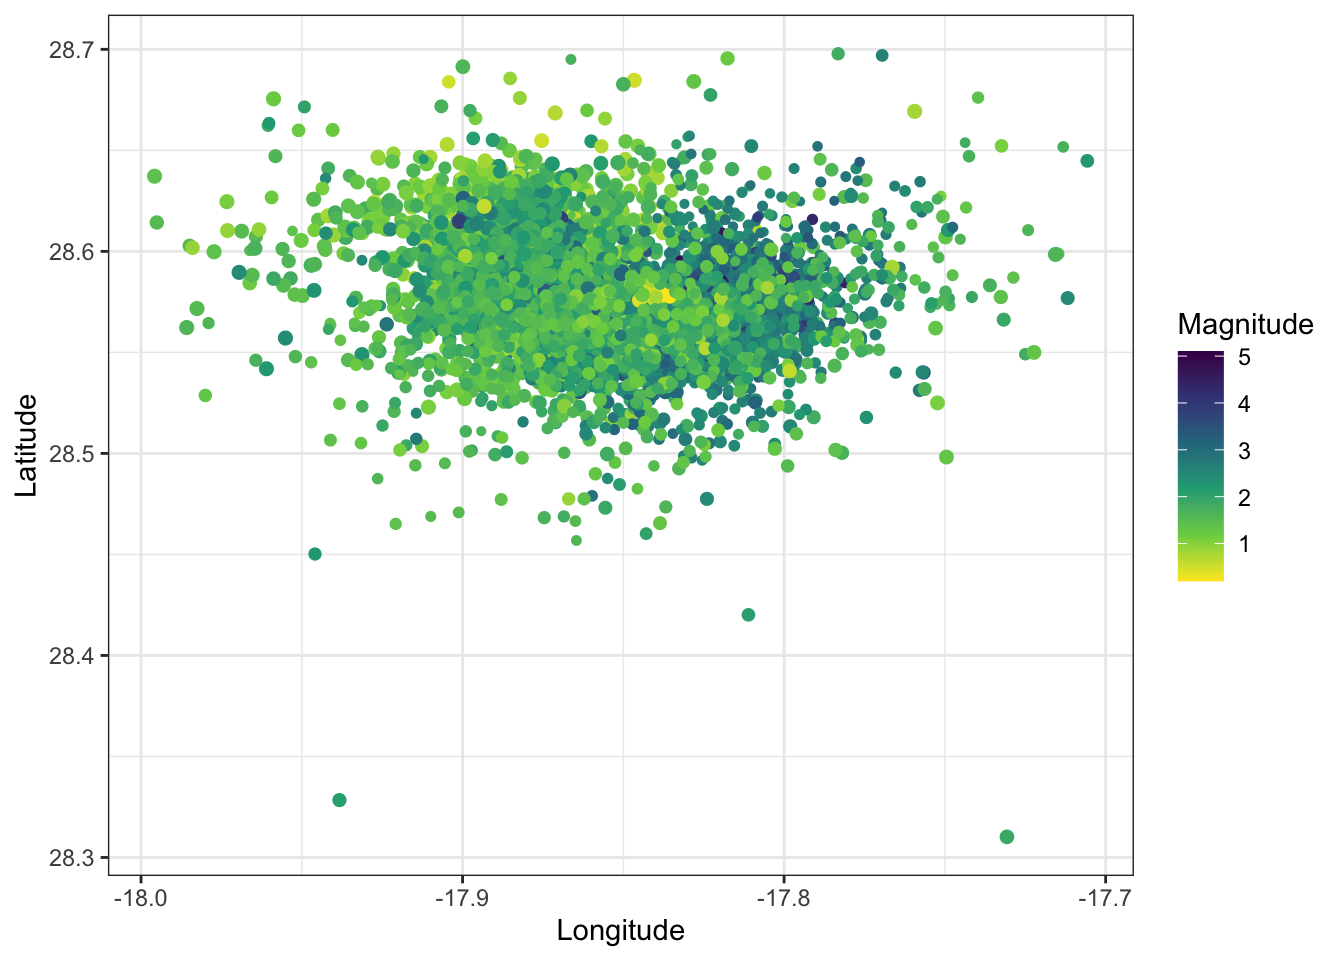
\includegraphics{index_files/figure-latex/notebooks-explore-earthquakes-fig-spatial-plot-output-1.png}

}

\caption{\label{fig-spatial-plot}Locations of earthquakes on La Palma
since 2017}

\end{figure}%

\textsubscript{Source:
\href{https://Scott-Akenhead.github.io/MS-Open-Salmon-KG/notebooks/explore-earthquakes-preview.html\#cell-fig-spatial-plot}{Explore
Earthquakes}}

Figure~\ref{fig-spatial-plot} shows the location of recent Earthquakes
on La Palma.

\section{Methods}\label{sec-methods}

\section{Results}\label{results}

\section{Conclusion}\label{conclusion}

\section{Acknowledgements}\label{acknowledgements}

\section{References}\label{references}

\phantomsection\label{refs}
\begin{CSLReferences}{1}{0}
\vspace{1em}

\bibitem[\citeproctext]{ref-archibald2021}
Archibald, D. W., McIver, R., \& Rangeley, R. (2021). Untimely
publications: Delayed Canadian fisheries science advice limits
transparency of decision-making. \emph{Marine Policy}, \emph{132},
104690. \url{https://doi.org/10.1016/j.marpol.2021.104690}

\bibitem[\citeproctext]{ref-chapman2019}
Chapman, K. (2019). First international year of the salmon data
laboratory (ISDL) workshop. In (Vol. 14, pp. 15--20). Vancouver, BC,
Canada. Retrieved from
\url{https://npafc.org/wp-content/uploads/technical-reports/Tech-Report-14/Technical-Report-14_Final.pdf}

\bibitem[\citeproctext]{ref-diack2023}
Diack, G., Bird, T., Akenhead, S., Bayer, J. M., Brophy, D., Bull, C.,
et al. (2023). Salmon data mobilization. Retrieved from
\url{https://osf.io/hk4gu}

\bibitem[\citeproctext]{ref-wilkinson2016}
Wilkinson, M. D., Dumontier, M., Aalbersberg, Ij. J., Appleton, G.,
Axton, M., Baak, A., et al. (2016). The FAIR guiding principles for
scientific data management and stewardship. \emph{Scientific Data},
\emph{3}(1), 160018. \url{https://doi.org/10.1038/sdata.2016.18}

\end{CSLReferences}



\end{document}
